\section{Preliminaries}
First, we introduce a couple of notions and definitions that will be used throughout this thesis. In particular, the definitions will play a crucial role in the theoretical part that follows. We start with some general notations, introduce a general graph definition, and familiarize the reader with the Weisfeiler-Leman algorithm. We will then introduce each framework independently, first the $\wlnn$ and then GNN. At the end, we will briefly introduce important properties of collections of functions computed by both methods.

\subsection{General Notation}
We first introduce a couple of notations and definitions that will be used throughout the thesis. With $[n]$, we denote the set $\{1, \ldots, n\} \subset \mathbb{N}$ for any $n \in \mathbb{N}$ and with $\MSopen \ldots \MSclose$ we denote a multiset which is formally defined as a 2 tuple $(X, m)$ with $X$ being a set of all unique elements and $m: X \rightarrow \mathbb{N}_{\geq 1}$ a mapping that maps every element in $X$ to its number of occurrences in the multiset.

\subsection{Graphs}
A graph $G$ is a 3-tuple $G\coloneqq (V, E, l)$ that consists of the set of all nodes $V$, the set of all edges $E \subseteq V \times V$ and a label function $l: M \rightarrow \Sigma$ with $M$ being either $V, V \cup E$ or $E$ and $\Sigma \subset \mathbb{N}$ a finite alphabet. Moreover, let $\mathcal{G}$ be the set of all finite graphs. Note that our definition of the labeling function allows graphs with labels either on the nodes only, on the edges only, or on both the nodes and the edges. In some cases we refer to the values assigned by $l$ as features instead of labels, however this is usually only the case when $\Sigma$ is multidimensional. In addition, although we have defined it this way, the labeling function is optional, and in cases where no labeling function is given, we add the trivial labeling function $f_1: V(G) \rightarrow \{1\}$.

Further, $G$ can be either directed or undirected, depending on the definition of $E$, where $E \subseteq \{(v,u) \mid v,u \in V\}$ defines a directed and $E \subseteq \{(v, u), (u,v) \mid v,u \in V, v\neq u\}$ such that for every $(v,u) \in E$ also $(u,v) \in E$ defines an undirected graph. Additionally, we will use the notation $V(G)$ and $E(G)$ to denote the set of nodes of $G$ and the set of edges of $G$ respectively, as well as $l_G$ to denote the label function of $G$. With $\mathcal{N}(v)$ for $v \in V(G)$ we denote the set of neighbors of $v$ defined as $\mathcal{N}(v) \coloneqq \{u \mid (u, v) \in E(G)\}$.

A coloring of a Graph $G$ is a function $C: V(G) \rightarrow \mathbb{N}$ that assigns each node in the graph a color (here a positive integer). Further, a coloring $C$ induces a partition $P$ on the set of nodes, for which we define $C^{-1}$ being the function that maps each color $c \in \mathbb{N}$ to its class of nodes with $C^{-1}(c) = \{ v\in V(G) \mid C(v) = c\}$. In addition, we define $h_{G, C}$ as the histogram of graph $G$ with coloring $C$, that maps every color in the image of $C$ under $V(G)$ to the number of occurrences. In detail, $\forall c \in \mathbb{N}: h_{G, C}(c) \coloneqq | \{ v \in V(G) \mid C(v) = c  \} | = | C^{-1}(c) |$

\subsubsection{Permutation-invariance and -equivariance}
We use $S_n$ to denote the symmetric group over the elements $[n]$ for any $n \in \Nb_{\geq 1}$. $S_n$ consists of all permutations over these elements. Let $G$ be a graph with $V(G) = [n]$, applying a permutation $\pi \in S_n$ on $G$, is defined as $G_\pi \coloneqq \pi \cdot G$ where $V(G_\pi) = \{\pi(1), \ldots, \pi(n) \}$ and $E(G_\pi) = \{ (\pi(v), \pi(u)) \mid (v,u) \in E(G)\}$. We will now introduce two key concepts for classifying functions on graphs.

\begin{definition}[Permutation Invariant]
    Let $f: \mathcal{G} \rightarrow \mathcal{X}$ be an arbitrary function, then $f$ is \textit{permutation-invariant} if and only if for all $G \in \mathcal{G}$ where $n_G \coloneqq \mid V(G) \mid$ and for every $\pi \in S_{n_G}$: $f(G) = f(\pi \cdot G)$.
\end{definition}

\begin{definition}[Permuation Equivariant]
    Let $f: \mathcal{G} \rightarrow \mathcal{X}$ be an arbitrary function, then $f$ is \textit{permuation-equivariant} if and only if for all $G \in \mathcal{G}$ where $n_G \coloneqq \mid V(G) \mid$ and for every $\pi \in S_{n_G}$: $f(G) = \pi^{-1} \cdot f(\pi \cdot G)$.
\end{definition}

\subsection{Weisfeiler and Leman Algorithm}\label{sec:1-WL Definition}
The Weisfeiler-Leman algorithm consists of two main parts, first the coloring algorithm and second the graph isomorphism test. We will introduce them in this section.

\subsubsection{The Weisfeiler-Leman graph coloring algorithm}
The $\wl$ algorithm computes a node coloring of its input graph in each iteration. A color for a node is computed using only the coloring of its neighbors and the node itself. The algorithm will continue as long as it has not converged, and returns the final coloring of the graph.

\begin{definition}[$\wl$ Algorithm]
Let $G = (V, E, l)$ be a graph, then in each iteration $i$, the 1-WL computes a node coloring $C_i: V(G) \rightarrow \mathbb{N}$. In iteration $i=0$, the initial coloring is $C_0 = l$ or if $l$ is non-existing $\forall v \in V(G): C_0(v) = c$ for an arbitrary constant $c \in \mathbb{N}$. For $i > 0$, the algorithm assigns a color to $v \in V(G)$ as follows:
\begin{equation*}
C_i (v) = \textsf{RELABEL}(C_{i-1}(v),  \ \MSopen C_{i-1}(u) \mid u \in \mathcal{N}(v) \MSclose),
\end{equation*}

\noindent where $\textsf{RELABEL}$ injectively maps the above pair to a unique, previously not used, natural number. The algorithm terminates when the number of colors between two iterations does not change, meaning the algorithm terminates after iteration $i$ if the following condition is satisfied:
\begin{equation*}
\forall v,w \in V(G):  C_i(v) = C_i(w) \iff C_{i+1}(v) = C_{i+1}(w).
\end{equation*}
Upon terminating we define $C_{\infty} \coloneqq C_i$ as the stable coloring, such that $\wl(G) \coloneqq C_\infty$.
\end{definition}


The colorings computed in each iteration always converge to the final one, such that the algorithm always terminates. In more detail, \cite{Gro2017} showed that it always holds after at most $|V(G)|$ iterations.
For an illustration of this coloring algorithm, see \autoref{Encoding example}. Moreover, based on the work of \cite{Pai+87} about efficient refinement strategies, \cite{Car+82} proved that the stable coloring $C_\infty$ can be computed in time $\mathcal{O}(| V(G) | + |E(G)| \cdot \log | V(G) |)$.

\subsubsection{The Weisfeiler-Leman Graph Isomorphism Test}

\begin{definition}[$\wl$ Isomorphism Test]
    To determine if two graphs $G, H \in \mathcal{G}$ are non-isomorphic ($G \ncong H)$, one applies the 1-WL coloring algorithm on both graphs ``in parallel'' and checks after each iteration if the occurrences of each color are equal, else the algorithm would terminate and conclude non-isomorphic. Formally, the algorithm concludes non-isomorphic in iteration $i$ if there exists a color $c$ such that: 
    \begin{equation*}
        |\{ v \in V(G) \mid c = C_i(v)\} | \neq |\{ v \in V(H) \mid c = C_i(v)\} |.
    \end{equation*}
\end{definition}
Note that this test is only sound and not complete for the \textit{graph isomorphism problem}. Counterexamples where the algorithm fails to distinguish non-isomorphic graphs can be easily constructed, see \autoref{1-WL Counter Example} which was discovered and proven by \cite{Cai1992}.
\begin{figure}[H]
    \centering
    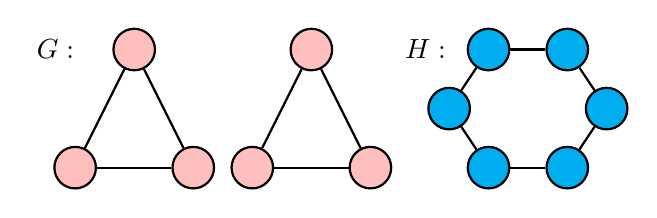
\begin{tikzpicture}

\tikzset{line/.style={draw,thick}}
\tikzset{arrow/.style={line,->,>=stealth}}
\tikzset{node/.style={circle,inner sep=0pt,minimum width=15pt}}

\draw (-1.0,0.75) node {$G:$};
\node[line,node,fill=pink] (x1) at (0, 0.75) {};
\node[line,node,fill=pink] (x2) at (-0.75, -0.75) {};
\node[line,node,fill=pink] (x3) at (0.75, -0.75) {};

\path[line] (x1) to (x2);
\path[line] (x1) to (x3);
\path[line] (x2) to (x3);

\node[line,node,fill=pink] (x1) at (2.25, 0.75) {};
\node[line,node,fill=pink] (x2) at (1.5, -0.75) {};
\node[line,node,fill=pink] (x3) at (3.0, -0.75) {};

\path[line] (x1) to (x2);
\path[line] (x1) to (x3);
\path[line] (x2) to (x3);

\draw (3.7, 0.75) node {$H:$};
\node[line,node,fill=cyan] (x1) at (3.75 + 0.25, 0) {};
\node[line,node,fill=cyan] (x2) at (4.25 + 0.25, 0.75) {};
\node[line,node,fill=cyan] (x3) at (5.25 + 0.25, 0.75) {};
\node[line,node,fill=cyan] (x4) at (5.75 + 0.25, 0) {};
\node[line,node,fill=cyan] (x5) at (5.25 + 0.25, -0.75) {};
\node[line,node,fill=cyan] (x6) at (4.25 + 0.25, -0.75) {};

\path[line] (x1) to (x2);
\path[line] (x2) to (x3);
\path[line] (x3) to (x4);
\path[line] (x4) to (x5);
\path[line] (x5) to (x6);
\path[line] (x6) to (x1);

\end{tikzpicture}
    \caption{An example of two graphs $G$ and $H$ that are non-isomorphic but cannot be distinguished by the 1-WL isomorphism test.}
    \label{1-WL Counter Example}
\end{figure}

\subsection{$\wlnn$}
As seen in the previous section, the $\wl$ algorithm is quite powerful in identifying substructures. With the $\wlnn$ framework, we define functions that utilize this structural information to derive further application-specific insights. We do this by combining well-known machine learning techniques and the algorithm.

\begin{definition}[$\wlnn$]
    We say a function $\cB$ working over a set of graphs $\cX \subseteq \cG$ is computable by $\wlnn$, if it can be decomposed into a multilayer perceptron $\mlp$, an encoding function $f_{enc}$ and the $\wl$ algorithm. In particular, when dealing with graph task $\cB$ can be decomposed as:
    \begin{align*}
        \cB: \cX \rightarrow \Rb, \ G \mapsto \text{MLP} \circ f_{\text{enc}}(\MSopen \wl(G)(v) \mid v \in V(G) \MSclose),
    \end{align*}
    where $\wl(G)$ is the coloring computed by the $\wl$ algorithm when applied on $G$. For node or edge tasks we define it as below:
    \begin{align*}
        \cB: \cX \rightarrow \mathcal{Y}, \ G \mapsto G' \coloneqq (V(G), \ E(G), \ \mlp \circ \wl(G)),
    \end{align*}
    where a graph $G$ is mapped to a structurally identical graph $G'$ with the key difference being that the label function is replaced with the coloring computed by the $\wl$ algorithm and further processed by a $\mlp$.
\end{definition}

As a concrete example of a collection of functions computable by $\wlnn$ we will introduce the collection of functions working from $\cX$ to $\Rb$ that use the so called \emph{counting-encoding} function as its encoding function.
We will define this particular encoding function in the following:

\begin{definition}[Counting Encoding Functions]\label{def:counting_encoding}
    The \emph{counting-encoding} function $f_{\text{count}, k}$ is parametrized by a $k \in \Nb$ and works as follows:
    \begin{equation*}
        f_{\text{count}, k}(\MSopen C(v)  \mid v \in V(G) \MSclose) := \begin{bmatrix}
            |\{ v \in V(G) \mid C(v) = 1 \}|\\
            \vdots\\
            |\{ v \in V(G) \mid C(v) = k \}|\\
        \end{bmatrix} \in \Nb^k.
    \end{equation*}
    It maps the occurrences of the colors $c \in [k]$ of its input to a vector over $\Nb^k$, such that each $i$.th component of this vector encodes the number of occurrences of the color $i$ in the input.
\end{definition}

To illustrate how this encoding function works and why we coined it \emph{counting-encoding}, we will quickly introduce an example graph $G$. In \autoref{Encoding example}, we give a visual representation of $G$ and its stable coloring after applying the 1-WL algorithm to it. The \emph{counting-encoding} function $f_{\text{count}, k}$ counts through all colors $i \in [k]$ and sets each $i$.th component of the output vector to the number of occurrences in the final coloring. Therefore, the respective color histogram $h_{G, C_\infty} = \MSopen 2, 2, 3, 4 \MSclose$ of $G$ is being mapped to $(0,2,1,1)^T \in \Nb^4$ by $f_{\text{count}, 4}$ and to $(0,2)^T \in \Nb^2$ by $f_{\text{count}, 2}$ for example, since color $2$ appears two times, while color $3$ and $4$ occur only once.
\begin{figure}[H]
    \centering
    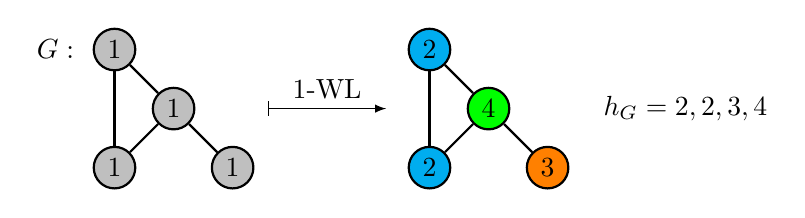
\begin{tikzpicture}
    \tikzset{line/.style={draw,thick}}
    \tikzset{arrow/.style={line,->,>=stealth}}
    \tikzset{node/.style={circle,inner sep=0pt,minimum width=15pt}}
    
    \draw (-1.5,0.75) node {$G:$};
    \node[line,node,fill=lightgray] (x1) at (-0.75, 0.75) {1};
    \node[line,node,fill=lightgray] (x2) at (-0.75, -0.75) {1};
    \node[line,node,fill=lightgray] (x3) at (0.75, -0.75) {1};
    \node[line,node,fill=lightgray] (x4) at (0, 0) {1};
    
    \path[line] (x1) to (x2);
    \path[line] (x1) to (x4);
    \path[line] (x2) to (x4);
    \path[line] (x3) to (x4);

    \draw [|-latex] (1.2,0) -- node [text width=2.5cm,midway,above,align=center ] {1-WL} (2.7,0);
    

    \node[line,node,fill=cyan] (x1) at (-0.75 + 4.0, 0.75) {2};
    \node[line,node,fill=cyan] (x2) at (-0.75 + 4.0, -0.75) {2};
    \node[line,node,fill=orange] (x3) at (0.75 + 4.0, -0.75) {3};
    \node[line,node,fill=green] (x4) at (0 + 4.0, 0) {4};
    
    \path[line] (x1) to (x2);
    \path[line] (x1) to (x4);
    \path[line] (x2) to (x4);
    \path[line] (x3) to (x4);

    \draw (6.5, 0.0) node {$h_G = \MSopen 2, 2, 3, 4 \MSclose$};

    
    
    \end{tikzpicture}

    \caption{An example of the final coloring computed by applying the 1-WL algorithm on the graph $G$. The graph $G$ consists of $4$ nodes with all their labels being initially set to $1$. Note that each label corresponds to a color, which we have also plotted for illustration purposes.}
    \label{Encoding example}
\end{figure}

\subsection{Graph Neural Networks (Message Passing)}\label{sec:GNN Defintion}
A Graph Neural Network (GNN) is a composition of multiple layers, where each layer computes a new feature for each node and edge. The GNN layer thus technically obtains a new graph that is structurally identical to the previous one, but contains new feature information. After an input graph has been passed through all layers, there can be an additional final function, aggregating the computed information into a fixed size output. With this, it is possible to apply a GNN to every graph, regardless of its size, as the ``computation'' will only take place on the nodes and edges of the graph.


Note that in the following we will restrict the definition to only consider node features, however, one can easily extend it to also include edge features.

\begin{definition}[Graph Neural Network]\label{def:gnn}
    Let $G = (V, E, l)$ be an arbitrary graph. A Graph Neural Network (GNN) is a composition of multiple layers where each layer $t$ is represented by a function $f^{(t)}$ that works over the set of nodes $V(G)$. To begin with, we need a function $f^{(0)}: V(G) \rightarrow \mathbb{R}^{1 \times d}$ that is consistent with $l$, that translates all labels into a vector representation. Further, for every $t > 0$, $f^{(t)}$ is of the format:
    \begin{align*}
    f^{(t)}(v) = f^{W_{1,t}}_{\text{merge}} (f^{(t-1)}(v), \  f^{W_{2,t}}_{\text{agg}}( \MSopen f^{(t-1)}(w) \mid w \in \mathcal{N}(v) \MSclose )),
    \end{align*}
    where $f^{W_{1,t}}_{\text{merge}}$ and $f^{W_{2,t}}_{\text{agg}}$ are arbitrary differentiable functions with $W_{1,t}$ and $W_{2,t}$ their respective parameters. Additionally, $f^{W_{2,t}}_{\text{agg}}$ has to be permuation-invariant.

    Depending on the objective, whether the GNN is tasked with a graph or a node task, the last layer differs. In the case of graph tasks, we add a permutation-invariant aggregation function to the end, here called $\textsf{READOUT}$, working as follows:
    \begin{align*}
        \textsf{READOUT}(\MSopen f^{(t)}(v) \mid v \in V(G) \MSclose),
    \end{align*}
    that aggregates over every node and computes a fixed-size output vector for the entire graph, e.g. a label for graph classification. In order to ensure that we can train the GNN in an end-to-end fashion, we require $\textsf{READOUT}$ to be also differentiable. Let $\mathcal{A}$ be an instance of the described GNN framework. Further, let $K \in \mathbb{N}$ be the number of layers of the GNN, $\mathcal{G}$ the set of all graphs, $\mathcal{Y}$ the task-specific output set (e.g. labels of a classification task), then the overall function computed by $\mathcal{A}$ is:
    \begin{align*}
        &\mathcal{A}: \mathcal{G} \rightarrow \mathcal{Y}, \ G \mapsto \textsf{READOUT}(\MSopen f^{(K)}(v) \mid v \in V(G) \MSclose),
    \end{align*}
    if $\mathcal{A}$ is configured for a graph task, otherwise:
    \begin{align*}
        &\mathcal{A}: \mathcal{G} \rightarrow \mathcal{Y}, \ G \mapsto G' \coloneqq (V(G), \ E(G), \ f^{(K)}),
    \end{align*}
    where a graph $G$ is mapped to a structurally identical graph $G'$ with the key difference being the label function is $f^{(K)}$.
\end{definition}

Note that, as we require all aggregation functions to be permutation-invariant, the total composition $\mathcal{A}$ is permutation-invariant, and with similar reasoning, it is also differentiable. This enables us to train $\mathcal{A}$ like any other machine learning method in an end-to-end fashion, regardless of the underlying encoding used for graphs. This definition and use of notation are inspired by \cite{Morris2018} and \cite{Xu2018}.

To demonstrate what kind of functions are typically used, we provide functions used by \cite{Ham+2017} for a node classification:
\begin{align*}
    f^{W_{1,t}}_{\text{merge}}(v) &= \text{ReLU} (W_{\text{merge}} \cdot \textsf{concat}(f^{(t-1)}(v), \ f^{W_{2,t}}_{\text{agg}}(v)))\\
    f^{W_{2,t}}_{\text{agg}}(v) &= \textsf{MAX}(\{ \text{ReLU}(W_{\text{pool}} \cdot f^{(t-1)}(u) + b) \mid u \in \mathcal{N}(v)\})
\end{align*}
where $\text{ReLU}$ is a rectified linear unit element wise activation function, $\textsf{MAX}$ the element-wise $\max$ operator; $W_{\text{merge}}$, $W_{\text{pool}}$ are trainable matrices, $b$ a trainable vector and \textsf{concat} the concatenation function.



\subsection{Important for later}
In this section, we introduce a formal definition of multilayer perceptron as it is required in a later proof, as well as the $\wliso$ relation. Additionally, two very important properties for collections of functions.

\begin{definition}[Multilayer Perceptron]\label{def:mlp}
    Multilayer perceptrons are a class of functions from $\Rb^n$ to $\Rb^m$, with $n,m \in \Nb$. In this thesis, we define a multilayer perceptron as a finite sequence, such that a multilayer perceptron $\mlp$ is defined as $\mlp \coloneqq (\mlp)_{i\in[k]}$ where $k$ is the number of layers. For every $i \in [k]$, the $i$.th layer of the $\mlp$ is the $i$.th item in the finite sequence $(\mlp)_i$. Further, all layers are recursively defined as:
    \begin{align*}
        (\mlp)_{0}(v) &\coloneqq v\\
        (\mlp)_{i+1}(v) &\coloneqq \sigma_i(W_i \cdot (\mlp)_{i} (v) + b_i), \quad \forall i \in [k-1]
    \end{align*}
    where $\sigma_i$ is an element wise activation function, $W_i$ is the weight matrix and $b_i$ the bias vector of layer $i$. Note, that for each $W_i$, the succeeding $W_{i+1}$ must have the same number of columns as $W_i$ has rows, in order to be well-defined. Similarly, for every layer $i$, $W_i$ and $b_i$ have to have the same number of rows.
    Following this definition, when applying a $\mlp$ on input $v \in \Rb^n$ it is $\mlp(v) \coloneqq (\mlp)_k(v)$.
\end{definition}

\begin{definition}[1-WL Relation]
    For any graphs $G,H \in \cX$ we will denote $G \wliso H$ if the 1-WL isomorphism test can not distinguish both graphs. Note that due to the soundness of this algorithm, if $G \not\wliso H$, we always can conclude that $G \not\simeq H$.
\end{definition}

The $\wliso$ relation can further be classified as an equivalence relation, as it is reflexive, symmetric and transitive. With this, we introduce a notation of its equivalence classes. Let $\cX \subseteq \cG$ and $G \in \cX$, then we denote with $\cX/\!{\wliso}(G): = \{ G' \in \cX \mid G \wliso G' \}$ its equivalence class.

\begin{definition}[$\wldisc$]
    Let $\mathcal{C}$ be a collection of permutation invariant functions from $\cX$ to $\Rb$. We say $\mathcal{C}$ is \textbf{\wldisc} if for all graphs $G_1, G_2 \in \mathcal{X}$ for which the 1-WL isomorphism test concludes non-isomorphic ($G_1 \not\wliso G_2$), there exists a function $h \in \mathcal{C}$ such that $h(G_1) \neq h(G_2)$.
\end{definition}

\begin{definition}[$\gapp$]
    Let $\mathcal{C}$ be a collection of permutation invariant functions from $\cX$ to $\Rb$. We say $\mathcal{C}$ is \textbf{\gapp} if for all permutation-invariant functions $\mathcal{A}$ computed by a GNN, and for all $\epsilon \in \Rb$ with $\epsilon > 0$, there exists $h_{\cA,\epsilon} \in \mathcal{C}$ such that $\| \cA - h_{\cA,\epsilon} \|_\infty \coloneqq \sup_{G \in \mathcal{X}} |\cA(G) - h_{\cA,\epsilon}(G)| < \epsilon$
\end{definition}

\section{Theoretical Connection}
This section is the main part of our theoretical investigation of the two frameworks. We will present 4 intriguing theorems, which will be proven separately afterwards. These results will form the basis for the empirical part that follows. The first two theorems will establish an equivalence between the two frameworks when the input set of graphs is finite. The last two theorems will go one step further and establish a connection for continuous functions computed by $\wlnn$ and GNNs and prove a somewhat weaker connection between them.

All the results we will now present focus on graph task functions, since this is the more complex problem, as any node or edge task function can be adapted to a graph task. In the first two theorems, we focus on a finite collection of graphs, which we denote by $\cX \subset \cG$.

\begin{theorem}[Finite Case: ``$\text{GNN} \subseteq \wlnn$'']\label{theorem:1wl_in_gnn}
    Let $\cC$ be a collection of functions from $\cX$ to $\Rb$ computable by GNNs, then $\cC$ is also computable by $\wlnn$.
\end{theorem}

\begin{theorem}[Finite Case: ``$\wlnn \subseteq \text{GNN}$'']\label{theorem:gnn_in_1wl}
    Let $\cC$ be a collection of functions from $\cX$ to $\Rb$ computable by $\wlnn$, then $\cC$ is also computable by GNNs.
\end{theorem}
With these theorems, we showed the equivalence between both frameworks. Specifically, every function computed by $\wlnn$ is also computable by a GNN, and vice versa. Notice that, we did not leverage any constraints on the encoding of graphs throughout the first two theorems and their corresponding proves, but rather kept it general. 

Having established a connection between the two frameworks on a finite subset of graphs, we wanted to further demonstrate the expressive power of $\wldisc$ by investigating a connection between the two frameworks for continuous feature spaces and continuous functions. However, since the graph isomorphism problem is an inherently discrete problem, the $\wl$ algorithm is only defined as a discrete and discontinuous function operating on discrete colors, such that extending the definition of the $\wl$ algorithm to a continuous function working over continuous values is not very trivial and, to our knowledge, has not yet been widely investigated. We therefore assume in the proofs and the following theorems that there exists a continuous version of the $\wl$ algorithm. 

We define the set of graphs with continuous features using the following definition:
\begin{definition}
    Let $X$ be a compact subset of $\Rb$ including $0$. We decode graphs with $n$ nodes as a matrix $G \in X^{n \times n}$, where $G_{i,i}$ decodes the label of node $i$ for $i \in [n]$, and $G_{i,j}$ with $i \neq j \in [n]$ decodes an edge from node $i$ to $j$ and a corresponding edge features. Furthermore, we say that there is an edge between node $i$ and $j$ if and only if $G_{i,j} \neq 0$. Additionally, if $G$ encodes an undirected graph, $G$ is a symmetric matrix. For simplicity, we denote $\cX \coloneqq X^{n \times n}$ throughout the next two theorems and their respective proofs.
\end{definition}

\begin{theorem}[Continuous Case: ``$\text{GNN} \subseteq \wlnn$'']\label{theorem:1wl_in_gnn_approximating}
    Let $\cC$ be a collection of continuous functions from $\cX$ to $\Rb$ computable by $\wlnn$. If $\cC$ is $\wldisc$, then there exists a collection of functions $\cC'$ computable by $\wlnn$ that is GNN-Approximating.
\end{theorem}

\begin{theorem}[Continuous Case: ``$\wlnn \subseteq \text{GNN}$'']\label{theorem:gnn_approximating_in_1wl}
    Let $\cC$ be a collection of continuous functions from $\cX$ to $\Rb$ that is GNN-Approximating, then $\cC$ is also $\wldisc$.
\end{theorem}

Since we only wanted to show the expressive power of $\wldisc$ and made the major assumption of the existence of a continuous $\wl$ algorithm, we have included the proofs of \cref{theorem:1wl_in_gnn_approximating,theorem:gnn_approximating_in_1wl} in the Appendix in \autoref{app:gnn_in_wlnn}.

Immediately from the last theorem follows the corollary:
\begin{corollary}
    There exists a collection $\cC$ of function from $\cX$ to $\Rb$ computable by GNNs that is $\wldisc$.
\end{corollary}

\begin{proof}
    The collection of all functions from $\cX$ to $\Rb$ computable by GNNs is trivially GNN-Approximating, such that we can apply \autoref{theorem:gnn_approximating_in_1wl} with which the proof concludes.
\end{proof}

By putting both theorems into perspective, we can now argue that even for continuous functions $\wlnn$ and GNNs can compute almost the same functions. Each framework can approximate the other framework arbitrarily well. From this we can conclude that the ability $\wldisc$ is very powerful, so we can assume that $\wlnn$ is sufficiently expressive for the upcoming empirical part.

\subsection{Proof of \autoref{theorem:1wl_in_gnn}}\label{sec:proof_theorem:1wl_in_gnn}
We will prove \autoref{theorem:1wl_in_gnn} by introducing a couple of small lemmas, which combined prove the theorem. In detail, in \autoref{lem:wl_disc_exists} we show the existence of a collection computed by $\wlnn$ that is 1-\!WL-Discriminating. In \cref{lem:wlnn_permutation_invariance,lem:wl_relation_equivalence,lem:composition_lemma} we derive properties of $\wlnn$ functions we will use throughout \cref{lem:encoding-indicator-func1,lem:encoding-indicator-func2,lem:decompose_gnn_as_wl} with which we prove the theorem.
We took great inspiration for \cref{lem:encoding-indicator-func1,lem:encoding-indicator-func2,lem:decompose_gnn_as_wl} from the proof presented in section 3.1 in the work of \cite{Chen2019}.

\begin{lemma}\label{lem:wl_disc_exists}
    There exists a collection $\cC$ of functions from $\cX$ to $\Rb$ computable by $\wlnn$ that is 1-\!WL-Discriminating.
\end{lemma}

\begin{proof}
    We define $f_c$  for $c \in \Nb$ as the encoding functions that returns the number of nodes colored as $c$. With this we can construct the collection of functions $C$ as follows:
    \begin{align*}
        C := \{ \cB_c: \cX \rightarrow \Rb, \ G \mapsto \mlp_\text{id} \circ f_c (\MSopen \wl(G)(v) \mid v \in V(G) \MSclose) \mid c \in \Nb\},
    \end{align*}
    where $\mlp_\text{id}$ is a dummy multilayer perceptron that just returns its input. Since every function $\cB_c \in C$ is composed of the $\wl$ algorithm, an encoding function and a multilayer perceptron, each function is computable by $\wlnn$, and consequently also the whole collection.

    Let $G_1, G_2 \in \cX$ with $G_1 \not\wliso G_2$. Further, let $C_1, C_2$ be the final colorings computed by the $\wl$ algorithm when applied on $G_1, G_2$
    respectively. Due to $G_1 \not\wliso G_2$, there exists a color $c \in \Nb$ such that $h_{G_1,C_1}(c)  \neq h_{G_2,C_2}(c)$. Such that $\cB_c \in C$ exists with $\cB_c(G_1) \neq \cB_c(G_2)$.
\end{proof}

\begin{lemma}[$\wlnn$ Equivalence]\label{lem:wl_relation_equivalence}
    Let $\cB$ be a function over $\cX$ computable by $\wlnn$, then for every pair of graphs $G_1, G_2 \in \cX:$ if $G_1 \wliso G_2$ than $\cB(G_1) = \cB(G_2)$.
\end{lemma}

\begin{proof}
    Let $\cB$ be an arbitrary function over $\cX$ computable by $\wlnn$, then $\cB$ is composed as follows: $\cB(\cdot) = \text{MLP} \circ f_{\text{enc}} \MSopen \wl(\cdot)(v) \mid v \in V(G) \MSclose$. Further, let $G_1, G_2 \in \cX$ be arbitrary graphs with $G_1 \wliso G_2$, then by definition of the relation $\wliso$ we know that $\wl(G_1) = \wl(G_2)$. With this the equivalence follows immediately.
\end{proof}

\begin{lemma}[$\wlnn$ Permuation Invariance]\label{lem:wlnn_permutation_invariance}
    Let $\cB$ be a function over $\cX$ computable by $\wlnn$, then $\cB$ is permutation invariant.
\end{lemma}

\begin{proof}
    Let $G_1, G_2 \in \cX$ be arbitrary graphs with $G_1 \simeq G_2$ and $\cB$ an arbitrary function computable by $\wlnn$. Since the $\wl$ algorithm is sound, we know that $G_1 \simeq G_2$ implies $G_1 \wliso G_2$. Using \autoref{lem:wl_relation_equivalence}, we can therefore conclude that: $\cB(G_1) = \cB(G_2)$.
\end{proof}

\begin{lemma}[$\wlnn$ Composition]\label[lemma]{lem:composition_lemma}
    Let $\cC$ be a collection of functions computable by $\wlnn$. Further, let $h_1, \dots h_n \in \cC$ and $\mlp^\bullet$ an multilayer perceptron, than the function $\cB$ composed of $\cB(\cdot) \coloneqq \mlp^\bullet(h_1(\cdot), \ldots, h_n(\cdot))$ is also computable by $\wlnn$.
\end{lemma}
\begin{proof}
    Assume the above and let $f_{1}, \ldots, f_{n}$ be the encoding functions, as well as $\text{MLP}_1, \ldots, \text{MLP}_n$ be the multilayer perceptrons used by $h_1, \dots h_n$ respectively. The idea of this proof is, we construct an encoding function $f^*$ that duplicates its input and applies each encoding function $f_i$ individually, and we construct a multilayer perceptron $\mlp^*$ that takes in this output and simulates all $\text{MLP}_1, \ldots, \text{MLP}_n$ simultaneously. Afterwards, the given $\mlp^\bullet$ will be applied on the concatenation of the output of all $\mlp_i$'s.  See \autoref{fig:proof_idea_parallelism} for a sketch of the proof idea. A complete proof can be found in the Appendix in \autoref{app:composition_proof}, as this proof is very technical and not that interesting.

    \begin{figure}[H]
        \centering
        \begin{tikzpicture}

    \tikzset{line/.style={draw,thick}}
    \tikzset{arrow/.style={line,->,>=stealth}}
    \tikzset{node/.style={circle,inner sep=0pt,minimum width=15pt}}
    
    \node (inputG) {$G$};
    \node (coloring) [right =of inputG] {$M_G$};
    \node (firstV) [right =of coloring] {$\begin{bmatrix*}
        f_1(M_G)\\
        \vdots\\
        f_n(M_G)
    \end{bmatrix*}$};
    \node (inp1) [above right =of firstV] {$f_1(M_G)$};
    \node (inp2) [below right =of firstV] {$f_n(M_G)$};
    \node (out1) [right =of inp1] {$o_1$};
    \node (out2) [right =of inp2] {$o_n$};
    \node (out) [below right =of out1, above right =of out2] {$\begin{bmatrix*}
        o_1\\
        \vdots\\
        o_n
    \end{bmatrix*}$};
    \node (dot1) [right =of firstV] {$\vdots$};
    \node (final_out) [right =of out] {$O$};
    \node (dot2) [below =of out1] {$\vdots$};

    

    \draw[|-latex] (inputG.east) to node[text width=2.5cm,midway,above,align=center] {$\wl$} (coloring.west);

    \draw[-latex] (coloring.east) to node[text width=2.5cm,midway,above,align=center] {$f^*$} (firstV.west);

    \draw[-latex] (firstV.east) -- (inp1.west);

    \draw[-latex] (firstV.east) -- (inp2.west);

    \draw[|-latex] (inp1.east) to node[text width=2.5cm,midway,above,align=center] {$\text{MLP}_1$} (out1.west);

    \draw[|-latex] (inp2.east) to node[text width=2.5cm,midway,above,align=center] {$\text{MLP}_n$} (out2.west);

    \draw[-latex] (out1.east) -- (out.west);
    \draw[-latex] (out2.east) -- (out.west);

    \draw[|-latex] (out.east) to node[text width=2.5cm,midway,above,align=center] {$\mlp^\bullet$} (final_out.west);

    %\draw [thick, decoration={brace,mirror,raise=0.5cm},decorate, below =of out2] (firstV.south) -- (final_out.west);


    %\draw (-1.5,0.75) node {$\cA(G):$};
    %\draw (-1.0, 0.0) node {$G$};

    %\draw [|-latex] (-0.6,0) -- node [text width=2.5cm,midway,above,align=center ] {1-WL} (1.0,0);

    %\draw (1.6, 0.0) node {$(M_G)_G$};

    %\draw [|-latex] (2.4, 0.0) -- node [text width=2.5cm,midway,above,align=center ] {$f$} (3.25, 0.0);
    
    %\draw (3.5, 0.0) node {$v$};

    %\draw (5.0, 1.0) node {$v$};
    %\draw (5.0, -1.0) node {$v$};
    
\end{tikzpicture}
        \caption{Proof idea for \autoref{lem:composition_lemma}, how the constructed functions $f^*$ and $\mlp^*$ will work on input $G$. Here we denote with $M_G$ the multiset of colors of the nodes of $G$ after the $\wl$ algorithm has been applied. More formally $M_G := \MSopen \wl(G)(v) \mid v \in V(G) \MSclose$. Further, we let $o_i$ be the output computed by $\mlp_i$ on input $f_i(M_G)$.}
        \label{fig:proof_idea_parallelism}
    \end{figure}
\end{proof}
    

\begin{lemma}\label[lemma]{lem:encoding-indicator-func1}
    Let $\cC$ be a collection of functions from $\cX$ to $\Rb$ computable by $\wlnn$ that is $\wldisc$. Then for all $G^* \in \cX$, there exists a function $h_{G^*}$ from $\cX$ to $\Rb$ computable by $\wlnn$, such that for all $G \in \cX: h_{G^*}(G) = 0$ if and only if $G \wliso G^*$.
\end{lemma}

\begin{proof}
    Assume the above. For any $G_1, G_2 \in \cX$ with $G_1 \not\wliso G_2$ let $h_{G_1, G_2} \in \cC$ be the function distinguishing them, with $h_{G_1, G_2}(G_1) \neq h_{G_1, G_2}(G_2)$. We define the function $\overline{h}_{G_1,G_2}$ working over $\cX$ as follows:
    \begin{align}\label{eq:lemma_inidcator_function_1}
        \overline{h}_{G_1, G_2}(\cdot) &= |h_{G_1, G_2}(\cdot) - h_{G_1, G_2}(G_1)| \nonumber\\
        &= \max(h_{G_1, G_2}(\cdot) - h_{G_1, G_2}(G_1), \ 0) + \max(h_{G_1, G_2}(G_1) - h_{G_1, G_2}(\cdot), \ 0) \nonumber\\
        &= \text{ReLU}(h_{G_1, G_2}(\cdot) - h_{G_1, G_2}(G_1)) + \text{ReLU}(h_{G_1, G_2}(G_1) - h_{G_1, G_2}(\cdot))
    \end{align}
    Note, that in the equations above ``$h_{G_1, G_2}(G_1)$'' is a fixed constant and the resulting function $\overline{h}_{G_1, G_2}$ is non-negative.
    Let $G_1 \in \cX$ now be fixed, we will construct the function $h_{G_1}$ with the desired properties as follows:
    \begin{align}\label{eq:lemma_inidcator_function_2}
        h_{G_1}(x) = \sum_{G_2 \in \cX, \ G_1 \not\wliso G_2} \overline{h}_{G_1, G_2}(x).
    \end{align}
    Since $\cX$ is finite, the sum is finite and therefore well-defined. Next, we will prove that for a fixed graph $G_1 \in \cX$, the function $h_{G_1}$ is correct on input $G \in \cX$:
    \begin{enumerate}
        \item If $G_1 \wliso G$, then for every function $\overline{h}_{G_1, G_2}$ of the sum with $G_1 \not\wliso G_2$, we know, using \autoref{lem:wl_relation_equivalence}, that $\overline{h}_{G_1, G_2}(G)$ is equal to $\overline{h}_{G_1, G_2}(G_1)$ which is by definition $0$, such that $h_{G_1}(G) = 0$.
        \item If $G_1 \not\wliso G$, then $\overline{h}_{G_1, G}(G)$ is a summand of the overall sum, and since $\overline{h}_{G_1, G}(G) > 0$, 
        we can conclude $h_{G_1}(G) > 0$ due to the non-negativity of each function $\overline{h}_{G_1, G_2}$.
    \end{enumerate}
    We can encode \autoref{eq:lemma_inidcator_function_1} via a multilayer perceptron where ``$h_{G_1, G_2}(G_1)$'' is just a constant, and consequently can encode \autoref{eq:lemma_inidcator_function_2} aswell. Therefore, we can conclude with \autoref{lem:composition_lemma} that for every graph $G$, $h_G$ is also $\wlnn$ computable.
\end{proof}

\begin{lemma}\label[lemma]{lem:encoding-indicator-func2}
    Let $\cC$ be a collection of functions from $\cX$ to $\Rb$ computable by $\wlnn$ so that for all $G^* \in \cX$, there exists $h_{G^*} \in \cC$ satisfying $h_{G^*}(G) = 0 $ if and only if $G \wliso G^*$ for all $G \in \cX$. Then for every $G^* \in \cX$, there exists a function $\varphi_{G^*} $ computable by $\wlnn$ such that for all $G \in \cX$: $\varphi_{G^*}(G) = \mathds{1}_{G \wliso G^*}$.
\end{lemma}
\begin{proof}
    Assuming the above. Due to $\cX$ being finite, we can define for every graph $G^*$ the constant:
    \begin{equation*}
        \delta_{G^*} \coloneqq \frac{1}{2} \min_{G \in \cX , \  G \not\wliso G^*} |h_{G^*}(G)| > 0.
    \end{equation*}
    With this constant, we can use a so-called ``bump'' function working from $\Rb$ to $\Rb$ that is similar to the indicator function. We define this function for parameter $a \in \Rb$ with $a > 0$ as:
    \begin{align}\label{eq:lemma_encoding_indicator_func2}
        \psi_a(x) &\coloneqq \max(\frac{x}{a} -1,\ 0) + \max(\frac{x}{a}+1, \ 0) - 2 \cdot \max(\frac{x}{a}, \ 0) \nonumber\\
        &= \text{ReLU}(\frac{x}{a} -1) + \text{ReLU}(\frac{x}{a}+1) - 2 \cdot \text{ReLU}(\frac{x}{a})
    \end{align}
    The interesting property of $\psi_a$ is that it maps every value $x$ to $0$, except when $x$ is being drawn from the interval $(-a, a)$. In particular, it maps $x$ to $1$ if and only if $x$ is equal to $0$. See \autoref{fig:bump_function} in the Appendix in \autoref{app:bump_function} for a plot of the relevant part of this function with exemplary values for $a$.
    
    We use these properties to define for every graph ${G^*} \in \cX$ the function $\varphi_{G^*}(\cdot) \coloneqq \psi_{\delta_{G^*}} (h_{G^*}(\cdot))$. 
    We will quickly demonstrate that this function is equal to the indicator function, for this let $G^*$ be fixed and $G$, an arbitrary graph from $\cX$, the input:
    \begin{enumerate}
        \item If $G \wliso G^*$, then $h_{G^*}(G) = 0$ resulting in $\varphi_{G^*}(G) = \psi_{\delta_{G^*}}(0) = 1$.
        \item If $G \not\wliso G^*$ then $h_{G^*}(G) \neq 0$, such that $|h_{G^*}(G)|> \delta_{G^*}$ so that $h_{G^*}(G) \not\in (-\delta_{G^*}, \delta_{G^*}) $ resulting in $\varphi_{G^*}(G) = 0$.
    \end{enumerate}
    Note that we can encode $\varphi_{G^*}$ using \autoref{eq:lemma_encoding_indicator_func2} via a multilayer perceptron, where $\delta_{G^*}$ is a constant. With \autoref{lem:composition_lemma} we can therefore conclude that $\varphi_{G^*}$ is computable by $\wlnn$ for every graph ${G^*} \in \cX$.
\end{proof}

\begin{lemma}\label{lem:decompose_gnn_as_wl}
    Let $\mathcal{C}$ be a collection of functions from $\cX$ to $\Rb$ computable by $\wlnn$ so that for all $G^* \in \cX$, there exists 
    $\varphi_{G^*} \in \cC$ satisfying $\forall G \in \cX: \varphi_{G^*}(G) = \mathds{1}_{G \wliso G^*}$, then every function computable by a GNN is also computable by $\wlnn$.
\end{lemma}

\begin{proof}
    Assume the above. For any function $\mathcal{A}$ computed by an GNN that works over $\cX$ to $\Rb$, we show that it can be decomposed as follows for any $G \in \cX$ as input:
    \begin{align}\label{eq:gnn_decomposition}
        \mathcal{A}(G) &= \Bigl( \ \frac{1}{|\cX/\!{\wliso}(G)|}\sum_{G^* \in \cX} \mathds{1}_{G \wliso G^*} \Bigr) \cdot \mathcal{A}(G) \nonumber \\
        &= \frac{1}{|\cX/\!{\wliso}(G)|}\sum_{G^* \in \cX} \mathcal{A}(G^*) \cdot \mathds{1}_{G \wliso G^*} \nonumber \\
        &= \sum_{G^* \in \cX} \frac{\mathcal{A}(G^*)}{|\cX/\!{\wliso}(G^*)|}  \cdot \varphi_{G^*}(G)
    \end{align}
    with $\cX/\!{\wliso}(G^*)$ we denote the set of all graphs $G$ over $\cX$ that are equivalent to $G^*$ according to the $\wliso$ relation.

    Since $\cA$ is permutation-invariant, and GNNs are at most as good as the 1-WL algorithm in distinguishing non-isomorphic graphs, we can use the fact that for every graph $G,H \in \cX$ with $G \wliso H$: $\cA(G) = \cA(H)$. Therefore, we can decompose $\cA$ as stated in \autoref{eq:gnn_decomposition} via a multilayer perceptron with $\frac{\cA(G^*)}{|\cX/\!{\wliso}(G^*)|}$ being constants and $\varphi_{G^*} \in \cC$ encoding the indicator function. Combined with the \autoref{lem:composition_lemma}, we can conclude that $\cA$ is computable by $\wlnn$. Important to note, we can only do this since $\cX$ is finite, making the overall sum finite and the cardinality of $\cX/\!{\wliso}(G^*)$ well-defined for all graphs.
\end{proof}

\subsection{Proof of \autoref{theorem:gnn_in_1wl}}
In this section we will prove the converse direction. We start with \cref{lem:1wl_color_upper_bound}, where we introduce an upper bound that we will use in \cref{lem:gnn_1wl_disc} to show that there exists a collection of GNN-computable functions that is $\wldisc$. After that, we will prove a composition lemma with \cref{lem:composition_lemma_gnn} which is similar to the one we introduced in the previous section. From this point on, the proof continues as in the previous section and concludes the property to be proved in \cref{lem:decompose_gnn_as_wl}.

\begin{lemma}\label{lem:1wl_color_upper_bound}
    Let $G$ be an arbitrary graph with $n \coloneqq |V(G)|$ the number of nodes and $C: V(G) \rightarrow \Nb$ an arbitrary coloring of the graph $G$. Then the total number of possible tuples of the form:
    \begin{equation*}
        (C(v), \ \MSopen C(u) \mid u \in \cN(v) \MSclose),
    \end{equation*}
    for all $v \in V(G)$ can be upper bounded by:
    \begin{equation*}
        n \cdot \sum_{i=0}^{n-1} \binom{n+i -1}{i}.
    \end{equation*}
\end{lemma}

\begin{proof}
    Assume the above. For the first entry of the tuple, there exist at most $n$ different colors, since there are $n$ nodes. For the second entry, each node $v \in V(G)$ can have between $0$ and $n-1$ neighbors, such that the total number of possibilities is the sum over each cardinality of a multiset with $n$ different colors. In the end, we soundly combine both results by multiplying both together.
\end{proof}


\begin{lemma}[GNN \wldisc]\label{lem:gnn_1wl_disc}
    There exists a collection $\cC$ of functions from $\cX$ to $\Rb$ computable by GNNs that is $\wldisc$. Meaning for every $G_1, G_2 \in \cX$ with $G_1 \not\wliso G_2$ there exists $\cA \in C$ such that $\cA(G_1) \neq \cA(G_2)$.
\end{lemma}

\begin{proof}
Since $\cX$ is finite, we define $n \coloneqq \max \{ |V(G)| \mid G \in \cX \}$ to be the maximum number of nodes of a graph in $\cX$, and $k \coloneqq \max \{ l_G(v) \mid v \in V(G), G \in \cX \}$ to be the largest label of any node of a graph in $\cX$. Using \cref{lem:1wl_color_upper_bound}, we can compute an upper bound $m$ using $n$ for the number of distinct tuples. Note that, this bound holds true for all graphs in $\cX$. We construct a GNN with $n$ layers working as follows for any $v \in V(G)$: 
\begin{align*}
    f^{(0)}(v) &\coloneqq l_G(v), \\
    f^{(t)}(v) &\coloneqq h_{m,t}(f^{(t-1)}(v), \ \MSopen f^{(t-1)}(u) \mid u \in \cN(v)\MSclose), \quad 0 < t < n.
\end{align*}
Here $h_{m,t}$ is a function that maps the tuples injectively to an integer of the set:
\begin{align*}\{i \in \Nb \mid k + (t-1)\cdot m +1 \leq i \leq k + t \cdot m\}
\end{align*}
such that each layer uses its own coloring domain. This function exists as by the soundness of the upper bound of \cref{lem:1wl_color_upper_bound} the cardinality of its co-domain is greater or equal than the one of its domain. With this, we ensure that each layer, maps a tuple to a new, previously not used, color. Therefore, every layer of this GNN, computes a single iteration of the $\wl$ algorithm. Further, since the $\wl$ algorithm converges after at most $|V(G)| =: n$ iterations, we set the number of layers to $n$. Thereby we ensure that the coloring computed after $n$ layers when applied on any graph $G \in \cX$ is similarly expressive as the coloring computed by the $\wl$ algorithm when applied on $G$.

We define the collection $C$ of functions computable by GNNs that is $\wldisc$ as: 
\begin{align*}
C \coloneqq \{ \cA: \cX \rightarrow \Rb, \ G \mapsto \textsf{Readout}_c(\MSopen f^{(n)}(v) \mid v \in V(G) \MSclose) \mid c \in \Nb \},
\end{align*}
where $\textsf{Readout}_c$ is the \textsf{READOUT} function that returns the number of nodes colored as $c$ in the coloring of $f^{(n)}$.
\end{proof}

Similar to the proof in the previous section, we will use \cref*{lem:composition_lemma_gnn} to introduce the ability to construct GNNs that take in as input multiple GNNs and then apply a multilayer perceptron to the combined output.


\begin{lemma}[Composition GNN]\label{lem:composition_lemma_gnn}
    Let $C$ be a collection of function computable by GNNs. Further, let  $\cA_1, \dots , \cA_n \in C$ and $\mlp$ a suitable multilayer perceptron, then \\$\hat{\cA}(\cdot) \coloneqq \mlp(\cA_1(\cdot), \dots, \cA_n(\cdot))$ is also computable by a GNN.
\end{lemma}

\begin{proof}
    Assume the above. Further, for the ease of readability we make the assumptions that the node features computed in each layer by each $\cA_i$ is one dimensional. Note that, one can easily extend this proof to work over arbitrary feature dimensions.

    Further, we will for any $x \in \Rb^d$ use the notation $x[i]$ to indicate the $i$.th element of the vector $x$. Also, we use the following notation to indicate the merge and aggregation function used in layer $t$ by $\cA_i$ as $f^{(t)}_{\text{merge}, i}$ and $f^{(t)}_{\text{agg}, i}$. Similarly, does $\textsf{Readout}_i$ indicate the \textsf{READOUT} function and $f^{(0)}_i$ the input function of $\cA_i$.
    
    We will prove the lemma by giving a construction of $\hat{\cA}$. Let $K$ be the maximum number of layers of all $\cA_1, \dots, \cA_n$. We construct the GNN $\hat{\cA}$ with $K$ layers, with the input layer working as follows on $v \in G$:
    \begin{align*}
        \hat{f}^{(0)}(v) \coloneqq \begin{bmatrix}
            f^{(0)}_1(v)\\
            \vdots\\
            f^{(0)}_n(v)
        \end{bmatrix},
    \end{align*}
    and each other layer $0 < t \leq K$ uses the merge $\hat{f}^{(t)}_{\text{merge}}$ and aggregation $\hat{f}^{(t)}_{\text{agg}}$ functions as defined below:
    \begin{align*}
        \hat{f}^{(t)}_{\text{merge}} (\hat{f}^{(t-1)}(v), \ Agg) &:= \begin{bmatrix}
            f^{(t)}_{\text{merge}, i}(\hat{f}^{(t-1)}(v)[1],\ Agg[1])\\
            \vdots\\
            f^{(t)}_{\text{merge}, n}(\hat{f}^{(t-1)}(v)[n],\ Agg[n])
        \end{bmatrix}\text{, and}\\
        \hat{f}^{(t)}_{\text{agg}}(\MSopen \hat{f}^{(t-1)}(w) \mid w \in \mathcal{N}(v) \MSclose ) &:= \begin{bmatrix}
            f^{(t)}_{\text{agg}, 1}(\MSopen f^{(t-1)}(w)[1] \mid w \in \mathcal{N}(v) \MSclose)\\
            \vdots\\
            f^{(t)}_{\text{agg}, n}(\MSopen f^{(t-1)}(w)[n] \mid w \in \mathcal{N}(v) \MSclose)
        \end{bmatrix}.
    \end{align*}
    Note that, not all $\cA_i$ will have $K$ layers. For these cases we define the missing functions as follows:
    \begin{align*}
        f^{(t)}_{\text{merge}, i}(\hat{f}^{(t-1)}(v), \ Agg) &\coloneqq \hat{f}^{(t-1)}(v)\text{, and}\\
        f^{(t)}_{\text{agg}, i}(\MSopen f^{(t-1)}(w) \mid w \in \mathcal{N}(v) \MSclose) &\coloneqq 0.
    \end{align*}
    These functions do not change anything, and only forward the result of the actual computation of $\cA_i$ to the last layer. Finally, we construct the \textsf{READOUT} function of $\hat{\cA}$ as follows:
    \begin{align*}
        \textsf{Readout}(\MSopen \hat{f}^{(t)}(v) \mid v \in V(G) \MSclose) \coloneqq \mlp \circ \begin{bmatrix}
            \textsf{Readout}_i(\MSopen f^{(t)}_{\text{merge}, 1}(v) \mid v \in V(G) \MSclose)\\
            \vdots\\
            \textsf{Readout}_n(\MSopen f^{(t)}_{\text{merge}, n}(v) \mid v \in V(G) \MSclose)
        \end{bmatrix}.
    \end{align*}
\end{proof}

As a result, we are in the same starting position as at the beginning of the proof in \autoref{sec:proof_theorem:1wl_in_gnn}. That is, we have shown with \cref{lem:gnn_1wl_disc} that there is a collection of functions that can distinguish any pair of graphs distinguishable by the 1-WL algorithm, and with \cref{lem:composition_lemma_gnn} we have shown that the composition of multiple GNNs and a multilayer perceptron is still computable by a GNN. Such that we can simply apply the results of \cref{lem:encoding-indicator-func1,lem:encoding-indicator-func2} to GNNs aswell and thereby concluding that for any fixed $G^* \in \cX$ the indicator function $\varphi_{G^*}$ working over $\cX$ with:
\begin{align*}
    \forall G \in \cX: \varphi_{G^*}(G) := \begin{cases}
    1, \quad \text{if $G \wliso G^*$}\\
    0, \quad \text{else}
\end{cases},
\end{align*}
is computable by a GNN.

\begin{lemma}\label{lem:decompose_gnn_as_wl}
    Let $\mathcal{C}$ be a collection of functions from $\cX$ to $\Rb$ computable by GNNs so that for all $G^* \in \cX$, there exists 
    $\varphi_{G^*} \in \cC$ satisfying $\forall G \in \cX: \varphi_{G^*}(G) = \mathds{1}_{G \wliso G^*}$, then every function computable by a $\wlnn$ is also computable by a GNN.
\end{lemma}

\begin{proof}
    Assume the above. For any function $\cB$ computed by $\wlnn$ that works over $\cX$ to $\Rb$, we show that it can be decomposed as follows for any $G \in \cX$ as input:
    \begin{align}\label{eq:1wl_decomposition}
        \cB(G) &= \Bigl( \ \frac{1}{|\cX/\!{\wliso}(G)|}\sum_{G^* \in \cX} \mathds{1}_{G \wliso G^*} \Bigr) \cdot \cB(G) \nonumber \\
        &= \frac{1}{|\cX/\!{\wliso}(G)|}\sum_{G^* \in \cX} \cB(G^*) \cdot \mathds{1}_{G \wliso G^*} \nonumber \\
        &= \sum_{G^* \in \cX} \frac{\cB(G^*)}{|\cX/\!{\wliso}(G^*)|}  \cdot \varphi_{G^*}(G)
    \end{align}
    with $\cX/\!{\wliso}(G^*)$ we denote the set of all graphs $G$ over $\cX$ that are equivalent to $G^*$ according to the $\wliso$ relation. With \cref{lem:wl_relation_equivalence}, we know that for any $G_1, G_2 \in \cX$ with $G_1 \wliso G_2: \cB(G_1) = \cB(G_2)$, such this decomposition is sound.
    
    
    We can encode $\cB$ as stated in \autoref{eq:1wl_decomposition} via a multilayer perceptron with $\frac{\cB(G^*)}{|\cX/\!{\wliso}(G^*)|}$ being constants and $\varphi_{G^*} \in \cC$ encoding the indicator function. Combined with the \autoref{lem:composition_lemma_gnn}, we can conclude that $\cB$ is computable by $\wlnn$. Important to note, we can only do this since $\cX$ is finite, making the overall sum finite and the cardinality of $\cX/\!{\wliso}(G^*)$ well-defined for all graphs.
\end{proof}



\newpage